\documentclass[working]{inputs/tuftebook}
\usepackage[utf8]{inputenc}
\usepackage[T1]{fontenc}
\usepackage{textcomp}

\usepackage{url}

\usepackage[
    sorting=nyt,
    style=alphabetic
]{biblatex}
\addbibresource{bibliography.bib}

\usepackage{hyperref}
\hypersetup{
    colorlinks,
    linkcolor={black},
    citecolor={black},
    urlcolor={blue!80!black}
}
\usepackage[noabbrev]{cleveref}

% Adds Bibliography, ... to Table of Contents
\usepackage[nottoc]{tocbibind}

\usepackage{graphicx}
\usepackage{float}
\usepackage[usenames,dvipsnames,svgnames]{xcolor}

% \usepackage{cmbright}

\usepackage{amsmath, amsfonts, mathtools, amsthm, amssymb}
\usepackage{mathrsfs}
\usepackage{cancel}

\newcommand\N{\ensuremath{\mathbb{N}}}
\newcommand\R{\ensuremath{\mathbb{R}}}
\newcommand\Z{\ensuremath{\mathbb{Z}}}
\renewcommand\O{\ensuremath{\emptyset}}
\newcommand\Q{\ensuremath{\mathbb{Q}}}
\newcommand\C{\ensuremath{\mathbb{C}}}
\let\implies\Rightarrow
\let\impliedby\Leftarrow
\let\iff\Leftrightarrow
\let\epsilon\varepsilon

\usepackage{tikz}
\usepackage{tikz-cd}

% theorems
\usepackage{thmtools}
\usepackage{thm-restate}
\usepackage[framemethod=TikZ]{mdframed}
\mdfsetup{skipabove=1em,skipbelow=0em, innertopmargin=12pt, innerbottommargin=8pt}

\theoremstyle{definition}

\makeatletter

\declaretheoremstyle[headfont=\bfseries\sffamily, bodyfont=\normalfont, mdframed={ nobreak } ]{thmgreenbox}
\declaretheoremstyle[headfont=\bfseries\sffamily, bodyfont=\normalfont, mdframed={ nobreak } ]{thmredbox}
\declaretheoremstyle[headfont=\bfseries\sffamily, bodyfont=\normalfont]{thmbluebox}
\declaretheoremstyle[headfont=\bfseries\sffamily, bodyfont=\normalfont]{thmblueline}
\declaretheoremstyle[headfont=\bfseries\sffamily, bodyfont=\normalfont, numbered=no, mdframed={ rightline=false, topline=false, bottomline=false, }, qed=\qedsymbol ]{thmproofbox}
\declaretheoremstyle[headfont=\bfseries\sffamily, bodyfont=\normalfont, numbered=no, mdframed={ nobreak, rightline=false, topline=false, bottomline=false } ]{thmexplanationbox}

\declaretheoremstyle[headfont=\bfseries\sffamily, bodyfont=\normalfont, numbered=no, mdframed={ nobreak, rightline=false, topline=false, bottomline=false } ]{thmexplanationbox}


\declaretheorem[numberwithin=chapter, style=thmgreenbox, name=Definition]{definition}
\declaretheorem[sibling=definition, style=thmredbox, name=Corollary]{corollary}
\declaretheorem[sibling=definition, style=thmredbox, name=Proposition]{prop}
\declaretheorem[sibling=definition, style=thmredbox, name=Theorem]{theorem}
\declaretheorem[sibling=definition, style=thmredbox, name=Lemma]{lemma}
\declaretheorem[sibling=definition, style=thmbluebox,  name=Example]{eg}
\declaretheorem[sibling=definition, style=thmbluebox,  name=Nonexample]{noneg}
\declaretheorem[sibling=definition, style=thmblueline, name=Remark]{remark}




\declaretheorem[numbered=no, style=thmexplanationbox, name=Proof]{explanation}
\declaretheorem[numbered=no, style=thmproofbox, name=Proof]{replacementproof}
\declaretheorem[style=thmbluebox,  numbered=no, name=Exercise]{ex}
\declaretheorem[style=thmblueline, numbered=no, name=Note]{note}

% \renewenvironment{proof}[1][\proofname]{\begin{replacementproof}}{\end{replacementproof}}

% \AtEndEnvironment{eg}{\null\hfill$\diamond$}%

\newtheorem*{uovt}{UOVT}
\newtheorem*{notation}{Notation}
\newtheorem*{previouslyseen}{As previously seen}
\newtheorem*{problem}{Problem}
\newtheorem*{observe}{Observe}
\newtheorem*{property}{Property}
\newtheorem*{intuition}{Intuition}


\declaretheoremstyle[
    headfont=\bfseries\sffamily\color{RawSienna!70!black}, bodyfont=\normalfont,
    mdframed={
        linewidth=2pt,
        rightline=false, topline=false, bottomline=false,
        linecolor=RawSienna, backgroundcolor=RawSienna!5,
    }
]{todo}
\declaretheorem[numbered=no, style=todo, name=TODO]{TODO}


\usepackage{etoolbox}
\AtEndEnvironment{vb}{\null\hfill$\diamond$}%
\AtEndEnvironment{intermezzo}{\null\hfill$\diamond$}%

% http://tex.stackexchange.com/questions/22119/how-can-i-change-the-spacing-before-theorems-with-amsthm
% \def\thm@space@setup{%
%   \thm@preskip=\parskip \thm@postskip=0pt
% }

\usepackage{xifthen}

\makeatother

% figure support (https://castel.dev/post/lecture-notes-2)
\usepackage{import}
\usepackage{xifthen}
\pdfminorversion=7
\usepackage{pdfpages}
\usepackage{transparent}


\makeatletter
\newif\ifworking
\@ifclasswith{tuftebook}{working}{\workingtrue}{\workingfalse}
\makeatother

\newcommand{\incfig}[2][1]{%
    % \ifworking{\makebox[0pt][c]{\color{gray}{\scriptsize\textsf{#2}}}}\fi%
    \def\svgwidth{#1\textwidth}
    \import{./figures/}{#2.pdf_tex}
}

\newcommand{\fullwidthincfig}[2][0.90]{%
    % \ifworking{\makebox[0pt][l]{\color{gray}{\scriptsize\textsf{#2}}}}\fi%
    \def\svgwidth{#1\paperwidth}
    \import{./figures/}{#2.pdf_tex}
}



\newcommand{\minifig}[2]{%
    \def\svgwidth{#1}%
    \begingroup%
    \setbox0=\hbox{\import{./figures/}{#2.pdf_tex}}%
    \parbox{\wd0}{\box0}\endgroup%
    \hspace*{0.2cm}
}

% %http://tex.stackexchange.com/questions/76273/multiple-pdfs-with-page-group-included-in-a-single-page-warning
\pdfsuppresswarningpagegroup=1

\newcommand\todo[1]{\ifworking {{\color{red}{#1}}} \else {}\fi}
\newcommand\charlotte[1]{\ifworking {{\color{blue}{#1}}} \else {}\fi}

\author{Gilles Castel}



\usepackage{multirow}
\def\block(#1,#2)#3{\multicolumn{#2}{c}{\multirow{#1}{*}{$ #3 $}}}

% \overfullrule=1mm

\newenvironment{myproof}[1][\proofname]{%
  \proof[\rm \bf #1]%
}{\endproof}

\usepackage{pdfpages}
\usepackage{efbox}


\usepackage{lipsum}
\usepackage{parskip}
\usepackage{titletoc}

\usepackage{cmbright}
\usepackage{bm}

\makeatletter
\newcommand{\globalcolor}[1]{%
  \color{#1}\global\let\default@color\current@color
}
\makeatother

\AtBeginDocument{\globalcolor{white}}

\definecolor{nord}{HTML}{313847}

\pagecolor{nord}


\begin{document}

\chapter*{Teori}
\subsubsection*{Snell's Law}
When light passes through a dielectrica, the angle of reflection is equal to the angle of incidence, whereas the angle refraction is given by Snell's law;
\begin{marginfigure}
    \incfig{snell}
    \caption{Depiction of Snell's Law. As the light crosses the barrier between the two dielectrica, its angle changes. This angle is called the \textit{angle of refraction}.}
    \label{fig:snell}
\end{marginfigure}
\[
	\boxed{n_a \sin \theta_a = n_b \sin \theta_b}
\]
Where $n_a$ and $n_b$ are known as the indexes of refraction, which are properties of different materials. A materials index of refraction $n$ is related to the speed at which light moves through the material.
\[
n = \frac{c}{v}
\]
\subsubsection{Polarized light}
An electromagnetic wave consists of an oscillating electric field and an oscillating magnetic field. Since these fields are perpendicular and the propagation direction is perpendicular to both fields it is a transverse wave. Every electromagnetic wave has a certain orientation in space which can be determined by using the right hand rule. This can also be used to find the polarization of the wave, where the direction of the electric field determines the polarization. E.g if the orientation of the electric field is in the y-direction the wave is called linearly polarized in the y-direction.
\\
The visible light emitted from natural light source such as a light bulb or a laser is unpolarized. This means that the light consists of waves that are polarized in every possible direction. The light can be polarized in a specific direction by using a device called a polarizer. This device acts as a filter allowing only waves polarized in a specific angle through. Relevant for this experiment is when putting a polarizer rotated to 45 degrees in front of the laser, the electric and magnetic field of the light passing through can be split into two equally large components.

\begin{marginfigure}
    \incfig{polarized}
    \caption{The top figure depicts S-polarized light, while the bottom figure depicts P-polarized light.}
    \label{fig:polarized}
\end{marginfigure}
\begin{marginfigure}
    \incfig{fresnel1}
    \caption{The proportion of light that is transmitted and reflected is described by Fresnel's relations. For both $S$- and $P$-polarized light, a greater proportion is transmitted for most angles. Notice, that when the dielectrica has a circular, the light can pass through without changing direction} 
    \label{fig:fresnel1}
\end{marginfigure}
\subsubsection{Brewster's angle}
At a specific angle determined by the index of refraction of the two materials, the reflected light is polarized in the perpendicular direction of the plane of incidence. The relation is given in Brewster's law for the polarizing angle:
\begin{align*}
    tan(\theta_p) = \frac{n_b}{n_a}
\end{align*}
\begin{marginfigure}
	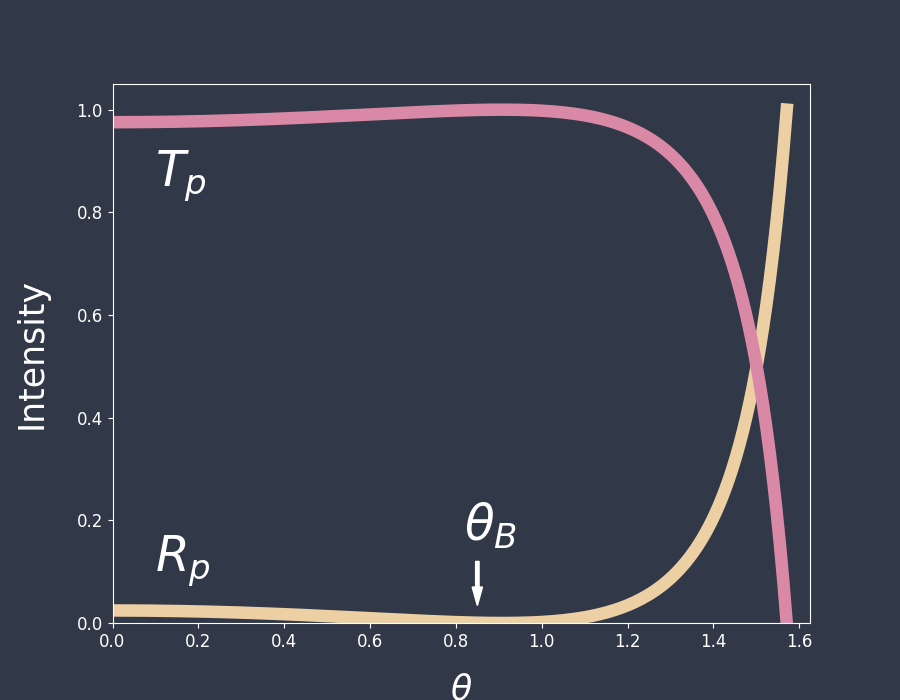
\includegraphics[width = 1.1\textwidth]{figures/fresnel2}
	\caption{This plot displays the intensities of the transmitted and reflected light. The transmitted light dominates for most angles. At tne brewster angle, all light is reflected. In this case, the index of refraction is 1.5 (glass).}
\end{marginfigure}
\subsubsection{The critical angle}
Another angle of interest is the critical angle, which can be derived from Snell's law of refraction by setting the refraction angle to 90 degrees:
\begin{align*}
    sin(\theta_{crit})=\frac{n_b}{n_a}
\end{align*}

At this angle no light is transmitted through the material. Instead the refracted light would move parallel with the demarcation line of the two materials. If the angle gets larger then total internal reflection occurs.
\subsubsection{Fresnel's Relations}
The angles of reflection and refraction are only part of the story. We are also interested in knowing how much of the incident light is reflected and transmitted. These intensities are given by the Fresnel relations, of which there are four. These relations describe the intensities of reflected and transmitted light for parallel and perpendicular polarized light. They have the following form;
\begin{align*}
	R_p &= \frac{\tan^2 \left( \theta_1 - \theta_2  \right) }{\tan^2 \left( \theta_1 + \theta_2  \right) }\\
	T_p &= \frac{sin(2\theta_1) sin(2\theta_2)}{sin^2(\theta_1+\theta_2)\cdot cos^2(\theta_1-\theta_2)}\\
	R_s &= \frac{\sin^2\left( \theta_1 - \theta_2 \right) }{\sin^2\left( \theta_1 + \theta_2 \right) } \\
	T_s &= \frac{sin(2\theta_1)sin(2\theta_2)}{sin^2(\theta_1 + \theta_2)}
.\end{align*}

If the energy is conserved then the sum of the intensity of all the different kinds of light should be equal to the intensity of the laser.
\begin{align*}
    T_p+T_s+R_p+R_s=I_{Laser}
\end{align*}
\begin{figure}[ht]
    \centering
    \incfig{fresnel3}
    \caption{fresnel3}
    \label{fig:fresnel3}
\end{figure}
\end{document}
